\PassOptionsToPackage{numbers, compress}{natbib}
\documentclass{article}
\usepackage[preprint]{neurips_2026}
\title{Step-Level Gradient Masking for GRPO:\\ Selective Optimization of Reasoning Trajectories}

\usepackage[utf8]{inputenc} 
\usepackage[T1]{fontenc}    
\usepackage[hidelinks]{hyperref}       
\usepackage{url}            
\usepackage{booktabs}       
\usepackage{amsfonts}       
\usepackage{nicefrac}       
\usepackage{microtype}      
\usepackage{xcolor}         
\usepackage{graphicx}
\usepackage{amsmath,amssymb}
\usepackage{algorithm}
\usepackage{algorithmic}
\usepackage{multirow}
\usepackage{float}


\workshoptitle{NewInML Workshop at NeurIPS 2026}

\author{%
  Youhan Lalwani \\
  Department of Artificial Intelligence \& Data Science \\
  Thadomal Shahani Engineering College \\
  \texttt{youhanlalwani@gmail.com} \\
  \And
  Mahesh Patel \\
  Department of Artificial Intelligence \& Data Science \\
  Thadomal Shahani Engineering College \\
  \texttt{patel2005mahesh@gmail.com} \\
  \And
  Himani Deshpande \\
  Department of Artificial Intelligence \& Data Science\\
  Thadomal Shahani Engineering College \\
  \texttt{himani.deshpande@thadomal.org} \\
}

\begin{document}

\maketitle

\begin{abstract}
Group Relative Policy Optimization (GRPO) has recently emerged as an effective algorithm for Reinforcement Learning from Verifiable Rewards (RLVR), allowing for improvements in logical reasoning, more specifically in mathematical reasoning in large language models (LLMs) without supervised reasoning traces. It does, however, face a credit assignment problem, in that it applies gradient updates uniformly across every token, including trivial formatting steps and already-mastered reasoning prefixes thereby wasting gradient capacity. We propose a step-level gradient masking framework for GRPO that restricts policy updates to structured reasoning steps where the model is still actively uncertain, instead of updating all tokens uniformly. The framework decomposes masking into three components: a step-generation protocol, a masking function, and a routing policy driven by a calibrated threshold. We instantiate the framework with two routing signals: \textbf{KL-GRPO} (KL-Divergence GRPO), which routes via per-step KL divergence from a reference model, and \textbf{EA-GRPO} (Entropy-Aware GRPO), which routes via the policy's own Shannon entropy and requires no reference model pass. Training Qwen3-4B on 2,000 stratified RLVR problems with Low-Rank Adaptation (LoRA), EA-GRPO achieves 72.94\% on MATH-500 (+1.04\% over standard GRPO, paired bootstrap $p=0.0423$) and 15.83\% on AIME 2025 (+2.83\%), while KL-GRPO attains the smoothest gradient trajectory and lowest format error rate (3.4\%). These results establish step-level gradient masking as a principled, low-overhead design point for GRPO-family training that improves generalization on hard mathematical reasoning tasks.
\end{abstract}



\section{Introduction}

The introduction of Reinforcement Learning from Verifiable Rewards (RLVR) has reshaped LLM training and fine-tuning for various tasks including but not limited to code generation, formatting and mathematical Reasoning. Methods such as DeepSeek-R1~\cite{Guo_2025} and subsequent GRPO-based systems~\cite{shao2024deepseekmath} have shown that verifiable reward signals, in which a symbolic checker confirms whether an answer is correct, can drive dramatic accuracy improvements without human-labeled reasoning traces. At the core of these methods is Group Relative Policy Optimization (GRPO)~\cite{shao2024deepseekmath}, which samples $k$ completions per input, computes group-relative advantages, and backpropagates gradients uniformly across every token in every trajectory. 

This uniform treatment, however, applies the same optimization pressure to tokens with substantially different learning signals. Early steps in mathematical reasoning chains, such as problem restatement, variable definition, and standard formula recall, often exhibit similar behavior across correct and incorrect trajectories and are typically generated with high model confidence. Thus, these steps have limited room for further improvement, while still receiving gradient updates. Moreover, such indiscriminate fine-tuning may also lead to entropy collapse~\cite{yu2025dapoopensourcellmreinforcement}, where repeated fine-tuning concentrates a model's output distribution around narrower, more formulaic responses.

The steps that should be reinforced are those where the model makes genuine decisions, like selecting computation strategies, evaluating competing simplification paths, or exploring a specific chain of reasoning. At these \emph{branching points}, gradient updates carry meaningful information about what reasoning works and what does not.

We implement this intuition through a \emph{step-level gradient masking framework} for GRPO. The framework outputs completions as reasoning steps, applies a masking function over these steps and then uses a routing policy to determine which step receives gradient updates. We present two instantiations of this framework that use reasoning steps as the smallest level of granularity instead of typical token-level approaches.

\textbf{KL-GRPO} (KL-Divergence GRPO) uses per-step KL divergence from the base model as the routing signal. Steps below the threshold are likely already base-model behavior implying suppressing their gradients prevents reinforcement of already-known content. \textbf{EA-GRPO} (Entropy-Aware GRPO) instead uses the policy's own per-step Shannon entropy. Steps where the model is already confident receive no gradient updates, whereas steps with high entropy (low confidence) receive the full gradient update.

Our contributions are:
\begin{enumerate}
    \item \textbf{A step-level gradient masking framework} for GRPO that is made up of three explicit components: step generation, a masking function, and a routing policy.
    \item \textbf{KL-GRPO} (KL-Divergence GRPO): an instantiation using per-step KL divergence as the routing signal, . with a precalibrated empirically determined threshold.
    \item \textbf{EA-GRPO} (Entropy-Aware GRPO): an instantiation using the policy's own Shannon entropy as a dynamic routing signal.
    \item \textbf{Empirical analysis}: a multi-run evaluation across three benchmarks showing that EA-GRPO yields improved accuracy on MATH-500 and AIME 2025, while KL-GRPO provides superior formatting preservation. We also identify an easy-hard trade-off in which step masking improves accuracy on high-difficulty problems at the expense of low-difficulty problems.
\end{enumerate}



\section{Related Work}

\textbf{RLVR and GRPO.} DeepSeek-R1~\cite{Guo_2025} has demonstrated that large language models can develop chain-of-thought reasoning through reinforcement learning with verifiable rewards (RLVR), without requiring human feedback. GRPO~\cite{shao2024deepseekmath} provides a lightweight policy-optimization framework for this setting by sampling multiple completions for each prompt and computing group-relative advantages from their rewards, avoiding the need for a separately learned value function. Subsequent work has shown that the basic GRPO formulation is susceptible to optimization pathologies and has proposed modifications to its clipping, sampling, normalization, and entropy behavior, including DAPO~\cite{yu2025dapoopensourcellmreinforcement} and Dr. GRPO~\cite{liu2025understandingr1zeroliketrainingcritical}. These developments motivate a broader question of how the learning signal produced by GRPO should be allocated within a long reasoning trajectory.

\textbf{Credit assignment in reasoning RL.} Outcome-based RLVR presents a fundamental credit-assignment challenge: GRPO derives an advantage from the final outcome of a sampled trajectory, yet a long reasoning trace contains many distinct decisions that may contribute differently to that outcome. Recent work has therefore explored finer-grained alternatives to trajectory-level credit. Segment Policy Optimization (SPO)~\cite{guo2025segmentpolicyoptimizationeffective} introduces segment-level advantage estimation as an intermediate granularity between trajectory-level GRPO and token-level policy optimization, seeking more precise credit assignment without relying on a learned critic. Other approaches similarly exploit structural or outcome-based information to redistribute credit within reasoning trajectories. These works suggest that the granularity at which learning signals are assigned is itself an important design choice for reasoning RL.

\textbf{Step-level structure in reasoning trajectories.} Reasoning trajectories are not homogeneous sequences of decisions: individual steps can differ substantially in difficulty, uncertainty, and their dependence on preceding reasoning. Consequently, a trajectory-level advantage may be incapable of distinguishing between steps which are already reliable and those that need further reinforcement. While credit can be assigned at different granularities, we focus on the reasoning step as a natural intermediate unit between the full trajectory and individual tokens. Step-level masking allows policy updates to be selectively applied to reasoning decisions while retaining the outcome-based learning signal of GRPO, providing finer control than trajectory-level optimization without requiring the granularity of token-level masking.




\section{Method}

\subsection{Preliminaries: GRPO}

Let $\pi_\theta$ denote the policy model and $\pi_\text{ref}$ the frozen reference model. For a prompt $q$, GRPO samples $k$ completions $\{o_1, \ldots, o_k\}$ and computes group-relative advantages:
\begin{equation}
A_i = \frac{r_i - \text{mean}(\mathbf{r})}{\text{std}(\mathbf{r}) + \varepsilon}
\label{eq:advantage}
\end{equation}
where $\mathbf{r} = \{r_1, \ldots, r_k\}$ are scalar rewards. The standard GRPO loss is:
\begin{equation}
\mathcal{L}_\text{GRPO} = -\mathbb{E}\!\left[\min\!\left(r_t A, \,\text{clip}(r_t, 1{-}\varepsilon, 1{+}\varepsilon) A\right)\right] + \beta \cdot \mathcal{L}_\text{KL}
\label{eq:grpo}
\end{equation}
where $r_t = \pi_\theta(a_t) / \pi_\text{old}(a_t)$ is the token-level importance ratio. This loss is applied identically to every token in every completion.

\subsection{Step-Level Gradient Routing Framework}

We propose \textbf{Step-Level Gradient Routing} (\textbf{SLGR}), a general framework for step-level gradient masking in GRPO that replaces the default uniform token weighting with a selective, step-granular masking policy. The framework has three distinct components:

\subsubsection{Step Generation}

Completions are structured so that the model outputs its chain-of-thought in discrete, programmatically detectable steps. While models can be fine-tuned to output this structure natively, in our instantiations we achieve step boundaries by instructing the model via system prompts to produce reasoning within \texttt{<think>} blocks, with each step enclosed in \texttt{<step>...</step>} tags, followed by a final response enclosed in \texttt{<answer>...</answer>}. LaTeX display equations are represented using \texttt{\$\$...\$\$} blocks. Step boundaries are detected by applying regular expressions to decoded completion text and mapping character-span offsets to token indices via the tokenizer's offset mapping. This yields an ordered list of token-index ranges $\{(s_1, e_1), (s_2, e_2), \ldots\}$ representing atomic reasoning steps. When no valid steps are detected, the mask defaults to all-ones and standard GRPO applies.

\subsubsection{Masking Function}
Given detected step boundaries and a routing decision, the masking function constructs a weight mask $M \in \{0,1\}^T$ over completion tokens. In our instantiations, we implement a \emph{Heaviside step function}: tokens prior to the first active step receive weight zero, while tokens from that step onward receive weight one. The gated loss is:
\begin{equation}
\mathcal{L}_\text{gated} = \frac{\sum_t M_t \cdot \mathcal{L}_t}{\sum_t M_t}
\label{eq:gated_loss}
\end{equation}
Alternative masking functions are possible within this framework, including soft gates that assign continuous weights to steps, threshold-based gates with a decay factor, or other continuous weighting functions based on signal magnitude. We select the Heaviside step gate for its simplicity, interpretability, and minimal hyperparameter footprint.

\subsubsection{Routing Policy}
The routing policy determines which detected steps are activated by evaluating a per-step scalar signal against a threshold parameter $\tau$. In our Heaviside implementation, $\tau$ directly controls the cutoff of this thresholding function and is treated as a hyperparameter rather than a learned parameter. We calibrate $\tau$ offline using the median of step statistics computed over \emph{divergent evaluation items}, which are problems where the baseline adapter and base model disagree on correctness, so that the threshold reflects the empirical distribution of the selected routing signal. We explore two specific routing signals below.

\subsection{Instantiation A: KL-GRPO (KL Divergence Routing)}

KL-GRPO uses per-step KL divergence from the reference model as its routing signal. For each step $s$, it computes:
\begin{equation}
\begin{split}
\text{KL}_s = \frac{1}{|s|} \sum_{t \in s} \Big[ &\exp\!\bigl(\log\pi_\text{ref}(a_t) - \log\pi_\theta(a_t)\bigr) \\
&- \bigl(\log\pi_\text{ref}(a_t) - \log\pi_\theta(a_t)\bigr) - 1 \Big]
\end{split}
\label{eq:step_kl}
\end{equation}

The threshold $\tau_\text{KL}$ is the \emph{median} of all per-step KL values across divergent items. The median is preferred over the mean because the KL distribution is right-skewed.

\textbf{Routing logic.} The active step $i^*$ is the first step where $\text{KL}_{s_{i^*}} > \tau_\text{KL}$. All tokens before $s_{i^*}$ are suppressed; all subsequent tokens receive the full gradient. Reference logits are reused from the KL regularization term already computed in the standard GRPO forward pass, adding no extra computation. If no step exceeds $\tau_\text{KL}$, or if fewer than two steps are detected, or if the advantage is zero, the mask defaults to all-ones (standard GRPO).

\subsection{Instantiation B: EA-GRPO (Entropy Routing)}

EA-GRPO uses the policy's own per-step Shannon entropy as the routing signal, requiring no reference model:
\begin{equation}
H_s = \frac{1}{|s|} \sum_{t \in s} \left[-\sum_{v \in \mathcal{V}} P(v \mid \mathbf{x}_t;\, \theta)\, \log P(v \mid \mathbf{x}_t;\, \theta)\right]
\label{eq:step_entropy}
\end{equation}
The threshold $\tau_H$ is the \emph{median} of per-step entropies across divergent items, chosen for robustness to the right-skewed entropy distribution. In our experiments, $\tau_H = 0.075$ nats.

\textbf{Routing logic.} The active step $i^*$ is the first step where $H_{s_{i^*}} \geq \tau_H$. Steps where the model is already confident (low entropy) are suppressed; steps where the model is uncertain receive the full update. Entropy is computed directly from the policy logits already present in the forward pass, introducing negligible overhead. Edge cases are handled identically to KL-GRPO.

\textbf{Comparison of routing signals.} KL divergence measures deviation from a static reference and can be increased by stylistic variations such as synonym choice, equation spacing, and step reordering that accumulate KL without reflecting genuine reasoning uncertainty. This may cause KL-GRPO to suppress updates on confident steps that merely phrase things differently from the reference. Shannon entropy is reference-free and measures only the sharpness of the policy's current output distribution, making it a more direct indicator of where the model is still uncertain. 

\begin{table}[!htbp]
\centering
\caption{Evaluation Accuracy (Mean \% $\pm$ Std Dev across runs)}
\label{tab:main_results}
\resizebox{\linewidth}{!}{%
\begin{tabular}{@{}lcccc@{}}
\toprule
\textbf{Dataset} & \textbf{Base Qwen3-4B} & \textbf{Baseline GRPO} & \textbf{KL-GRPO (KL)} & \textbf{EA-GRPO (Entropy)} \\
\midrule
MATH-500 (25 runs) & 68.42\,{\scriptsize$\pm$1.33} & 71.90\,{\scriptsize$\pm$1.10} & 71.85\,{\scriptsize$\pm$0.83} & \textbf{72.94\,{\scriptsize$\pm$1.11}} \\
AIME 2025 (20 runs) & 13.50\,{\scriptsize$\pm$4.77} & 13.00\,{\scriptsize$\pm$3.57} & 14.00\,{\scriptsize$\pm$3.99} & \textbf{15.83\,{\scriptsize$\pm$5.50}} \\
GSM8K (10 runs) & 90.36\,{\scriptsize$\pm$0.40} & \textbf{90.86\,{\scriptsize$\pm$0.38}} & 90.67\,{\scriptsize$\pm$0.48} & 90.60\,{\scriptsize$\pm$0.43} \\
\bottomrule
\end{tabular}%
}
\end{table}



\section{Experimental Setup}

\subsection{Model and Fine-Tuning}

We use \textsc{Qwen3-4B}~\cite{yang2025qwen3technicalreport} as the base model, selected for its strong mathematical reasoning baseline and VRAM-efficient inference footprint. All three variants are trained with Low-Rank Adaptation (LoRA)~\cite{hu2021loralowrankadaptationlarge} to keep the training tractable on a single GPU. The LoRA configuration targets all linear projection layers (\texttt{q\_proj}, \texttt{k\_proj}, \texttt{v\_proj}, \texttt{o\_proj}, \texttt{gate\_proj}, \texttt{up\_proj}, \texttt{down\_proj}) with rank $r=32$, $\alpha=64$, dropout $0.05$. All experiments were conducted on a single NVIDIA L40S GPU (48 GB VRAM) hosted through RunPod.

\subsection{Training Data}

Training data consists of 2{,}000 problems sub-sampled from the \textbf{AllenAI RLVR Math} dataset~\cite{allenairlvr2025}, stratified across seven subjects (Algebra, Geometry, Number Theory, Precalculus, Intermediate Algebra, Counting \& Probability, Prealgebra) and five difficulty levels to ensure balanced representation. This restricted scale reflects GPU compute budget constraints; we discuss scaling implications in Section~\ref{sec:limits}.

\subsection{Reward Function}

We use a compound scalar reward $r \in [0.0, 1.0]$:
\begin{equation}
\begin{aligned}
r =\;& \underbrace{0.85 \cdot \mathbb{I}[\text{correct}]}_{r_\text{acc}\text{ (reasoning)}} \\
&+\; \underbrace{0.05 \cdot \mathbb{I}[\text{think}] + 0.05 \cdot \mathbb{I}[\text{answer}] + 0.05 \cdot \mathbb{I}[\text{step}\ge 2]}_{r_\text{fmt}\text{ (format)}}
\end{aligned}
\label{eq:reward}
\end{equation}
Answer correctness is verified via a four-tier cascade: exact string matching after LaTeX normalization, numerical float comparison (tolerance $< 10^{-2}$), and SymPy symbolic simplification via both \texttt{parse\_latex} and \texttt{sympify}.

\subsection{GRPO Hyperparameters}

All three variants share identical GRPO hyperparameters: group size $k=4$, KL coefficient $\beta=0.01$, clip epsilon $\varepsilon=0.2$, learning rate $10^{-5}$, maximum new tokens 1{,}024, generation temperature 0.7, top-$p$ 0.9, gradient clipping norm 1.0, batch size 2 with 2 gradient accumulation steps. Generation is accelerated via vLLM~\cite{kwon2023efficientmemorymanagementlarge} in colocate mode. Training runs for 2{,}001 steps with checkpoints saved every 200 steps. Table~\ref{tab:hyperparams} summarizes hyperparameter values.

\begin{table}[!htbp]
\centering
\caption{Hyperparameter Configuration}
\label{tab:hyperparams}
\begin{tabular}{@{}lc@{}}
\toprule
\textbf{Hyperparameter} & \textbf{Value} \\
\midrule
Base model & Qwen3-4B \\
LoRA rank / alpha & 32 / 64 \\
Trainable parameters & $\approx$0.3\% \\
Group size $k$ & 4 \\
KL coefficient $\beta$ & 0.01 \\
Clip $\varepsilon$ & 0.2 \\
Learning rate & $1 \times 10^{-5}$ \\
Max new tokens & 1{,}024 \\
Temperature (training) & 0.7 \\
Training steps & 2{,}001 \\
KL-GRPO $\tau_\text{KL}$ & 0.0009 \\
EA-GRPO $\tau_H$ & 0.075 nats \\
\bottomrule
\end{tabular}
\end{table}

\subsection{Evaluation Protocol}

To suppress stochastic variance, each adapter is evaluated in multiple independent runs at temperature 0.7 with $\texttt{max\_tokens} = 2{,}048$ (MATH-500~\cite{hendrycks2021measuringmathematicalproblemsolving}, GSM8K~\cite{cobbe2021trainingverifierssolvemath}) or $4{,}096$ (AIME). Run counts are: MATH-500: 25 runs (12{,}500 evaluations per model); GSM8K: 10 runs (13{,}190 evaluations); AIME 2025: 20 runs (600 evaluations). We report mean accuracy and standard deviation across runs. Evaluation uses the same answer-matching cascade as training.



\section{Results}

\subsection{Main Accuracy Results}

Table~\ref{tab:main_results} summarizes mean accuracy and standard deviation across all stochastic evaluation runs. To further characterize result reliability, Figure~\ref{fig:ci} reports 95\% confidence intervals computed via the t-distribution across all runs per model per benchmark. EA-GRPO is the strongest overall performer on the harder benchmarks, while all three fine-tuned models saturate GSM8K.

On MATH-500, EA-GRPO achieves 72.94\% (95\%~CI: $\pm$0.46\%), representing a $+$2.52\% absolute gain over the base model and $+$1.04\% over Baseline GRPO. The improvement is even more pronounced on AIME 2025, where EA-GRPO reaches 15.83\% (95\%~CI: $\pm$2.57\%) versus 13.00\% ($\pm$1.67\%) for Baseline GRPO and 14.00\% ($\pm$1.87\%) for KL-GRPO, a $+$2.83\% gain over the baseline on a 30-problem Olympiad benchmark. On GSM8K, all adapted models cluster within 0.5\% of each other, consistent with near-saturation at $\approx$90.6\%.

\subsection{Statistical Significance: Paired Bootstrap Test}
\label{sec:bootstrap_app}
To verify that EA-GRPO's MATH-500 advantage is not attributable to evaluation variance, we conduct a paired bootstrap significance test over the per-problem evaluation logs. Per-problem mean correctness is averaged across all 25 stochastic evaluation runs, yielding paired vectors $\mathbf{a}_{\text{EA}},\mathbf{a}_{\text{Base}}\!\in\![0,1]^{500}$. The test statistic $\delta_\text{obs}=\overline{\mathbf{a}_{\text{EA}}}-\overline{\mathbf{a}_{\text{Base}}}$ is compared against $B=10{,}000$ bootstrap resamples of 500 problem indices drawn with replacement. The one-sided $p$-value is the fraction of resamples where $\delta_b\leq 0$; $p=0.0423<0.05$ confirms statistical significance (Table~\ref{tab:bootstrap_app}).

\begin{table}[!htbp]
\centering
\caption{Paired Bootstrap Test: EA-GRPO vs.\ Baseline GRPO on MATH-500 ($B=10{,}000$ resamples, 25 evaluation runs per model).}
\label{tab:bootstrap_app}
\small
\begin{tabular}{@{}lr@{}}
\toprule
\textbf{Metric} & \textbf{Value} \\
\midrule
Problems $N$                  & 500 \\
Evaluation runs per model     & 25 \\
Bootstrap resamples $B$       & 10{,}000 \\
Baseline GRPO mean acc.       & 71.90\% \\
EA-GRPO mean acc.             & 72.94\% \\
Observed $\delta$             & $+$1.04\% \\
Bootstrap std.\ of $\delta$  & 0.60\% \\
95\% Bootstrap CI             & $[-0.13\%, +2.25\%]$ \\
$p$-value (one-sided)         & \textbf{0.0423} \\
\bottomrule
\end{tabular}
\end{table}

\begin{figure*}[!htbp]
\centering
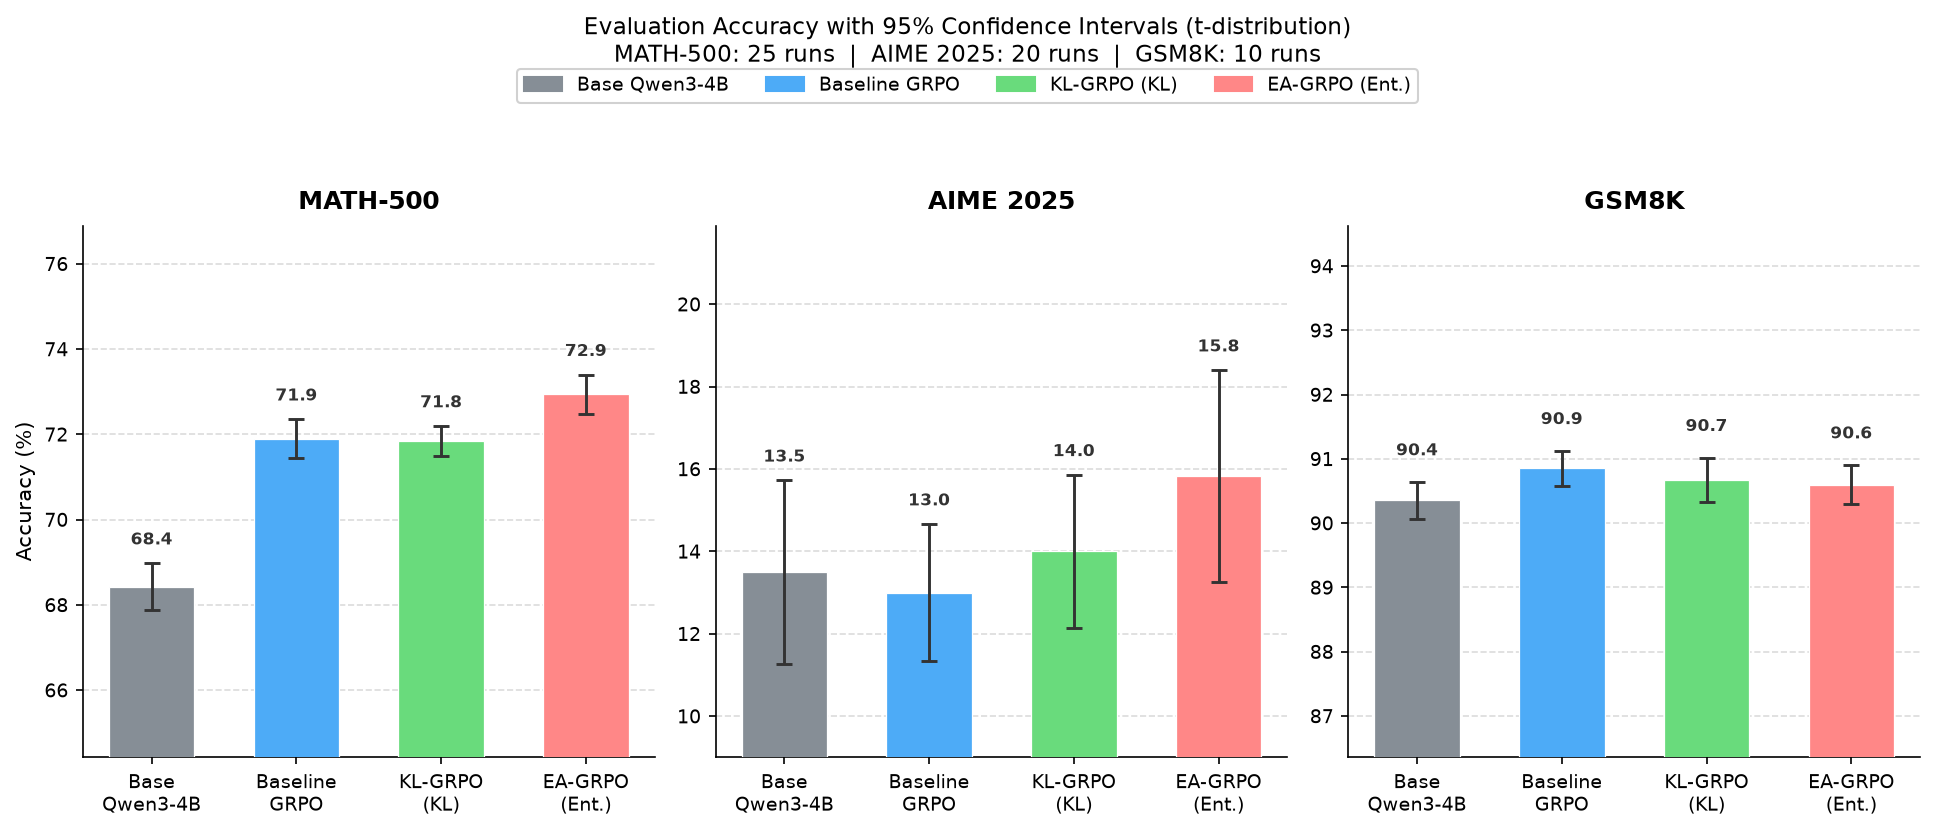
\includegraphics[width=0.92\textwidth]{images/ci_accuracy_comparison.png}
\caption{Evaluation accuracy with 95\% confidence intervals (t-distribution) across all models and benchmarks.}
\label{fig:ci}
\end{figure*}

\subsection{Difficulty-Level and Subject Breakdown}

Table~\ref{tab:difficulty} breaks MATH-500 performance down by difficulty level. On easy problems (Level 1--2), Baseline GRPO outperforms both masked variants; on hard problems (Level 3--5), EA-GRPO is consistently superior.

\begin{table}[h]
\centering
\caption{MATH-500 Accuracy by Difficulty Level (\%)}
\label{tab:difficulty}
\begin{tabular}{@{}lrcccc@{}}
\toprule
\textbf{Level} & \textbf{N} & \textbf{Base} & \textbf{Baseline} & \textbf{KL-GRPO} & \textbf{EA-GRPO} \\
\midrule
Level 1 & 43  & 86.42 & \textbf{89.58} & 88.47 & 88.09 \\
Level 2 & 90  & 83.47 & \textbf{87.64} & 85.42 & 84.84 \\
Level 3 & 105 & 78.78 & 80.95 & 81.94 & \textbf{83.50} \\
Level 4 & 128 & 67.44 & 70.84 & 72.53 & \textbf{73.75} \\
Level 5 & 134 & 45.37 & 49.55 & 48.84 & \textbf{51.01} \\
\bottomrule
\end{tabular}
\end{table}

EA-GRPO achieves its largest gains at Level 5 ($+$5.64\% over Base, $+$1.46\% over Baseline) and Level 4 ($+$6.31\% over Base). The Baseline GRPO advantage on Level 1--2 reflects a fundamental trade-off: uniform gradient updates across all tokens cause the model to disproportionately optimize for simple, high-frequency patterns, improving performance on easy problems at the cost of hard-problem capacity. Step masking reverses this allocation.

\subsection{Training Dynamics and Gradient Stability}

Figure~\ref{fig:gradnorm} shows the per-step L2 gradient norm on a log scale. KL-GRPO's KL-based masking produces the most stable gradient profile by filtering out low-KL formatting and boilerplate tokens before they contribute to the gradient.

\begin{figure}[h]
\centering
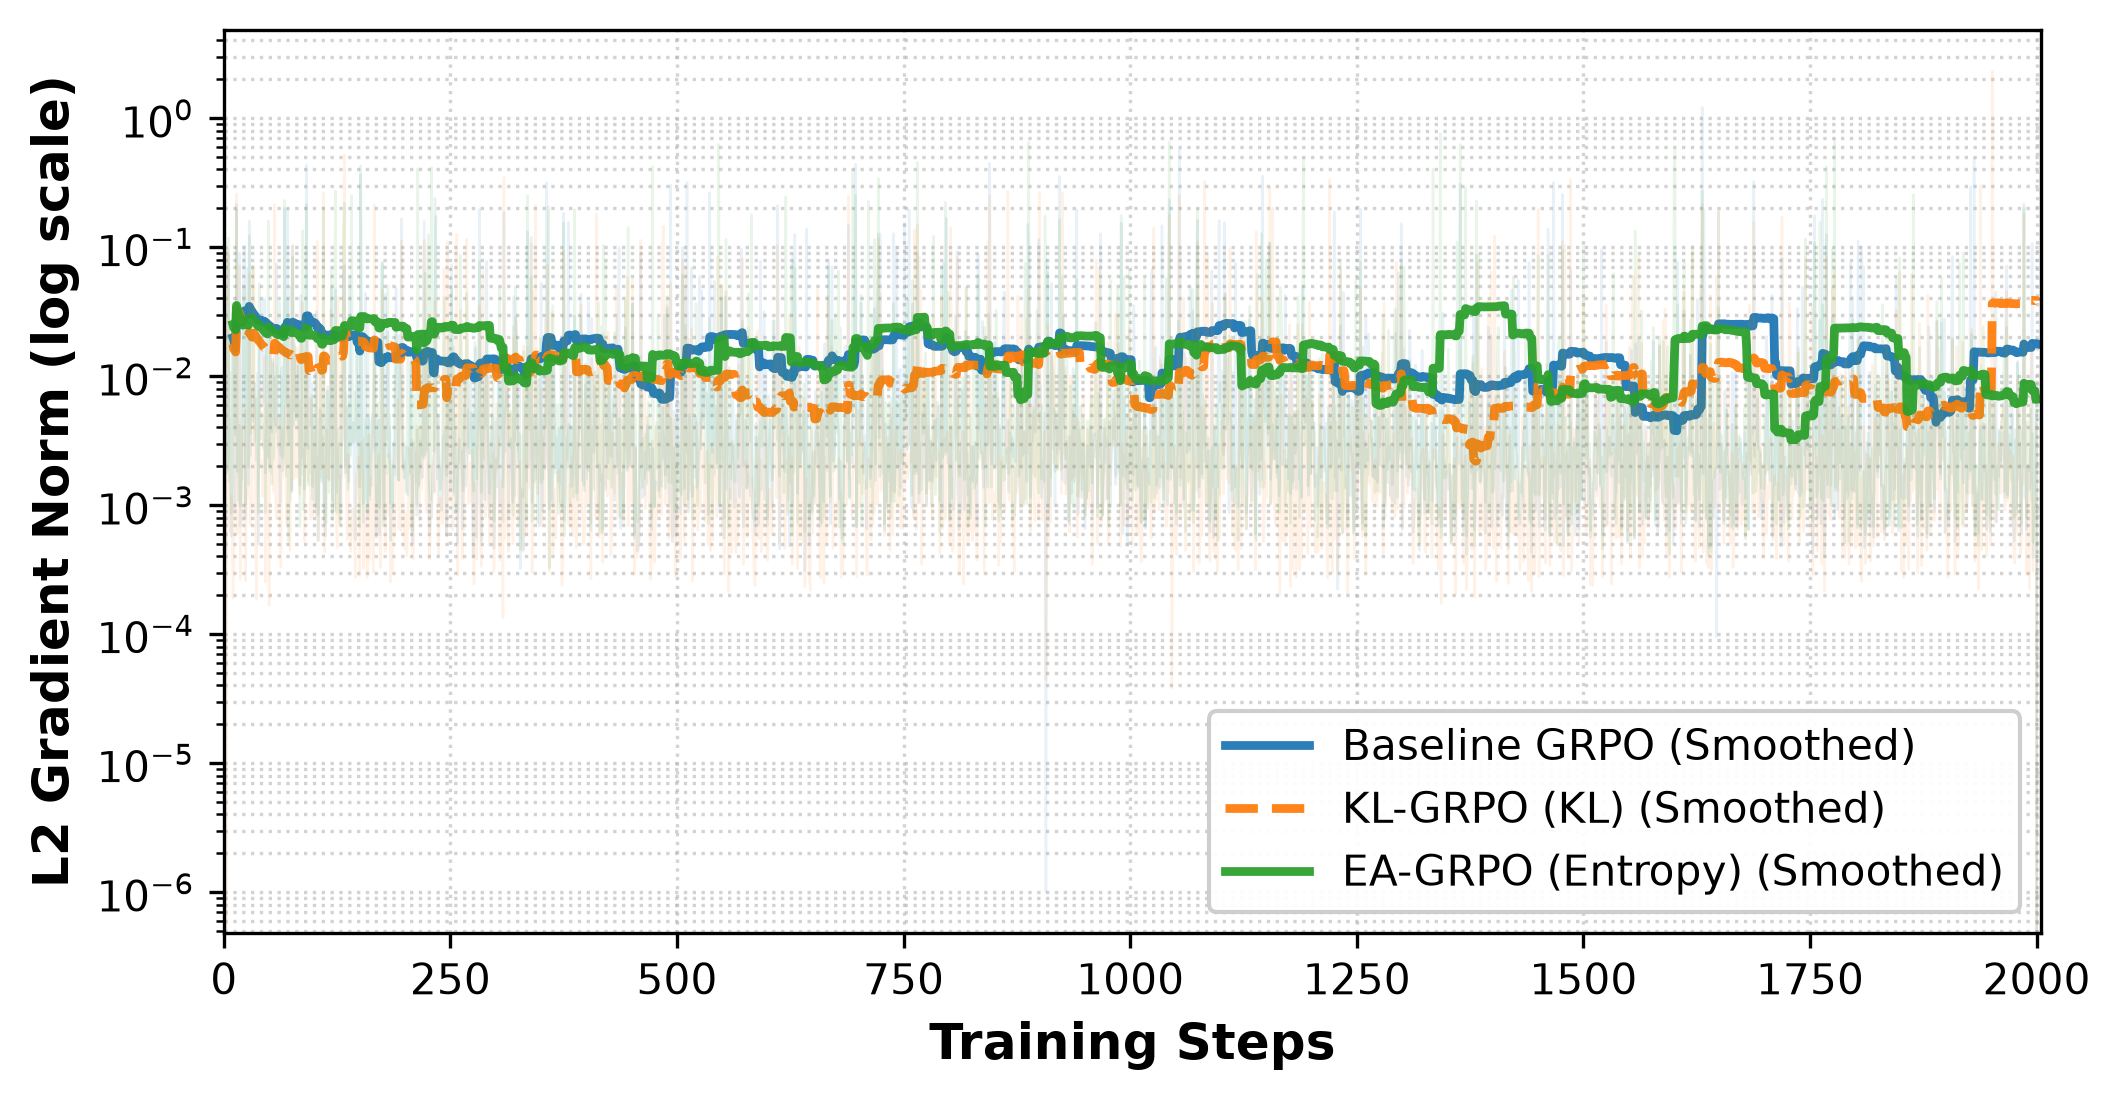
\includegraphics[width=0.85\linewidth]{images/gradient_norm_stability.png}
\caption{LoRA L2 gradient norm over training (log scale, rolling mean).}
\label{fig:gradnorm}
\end{figure}

\begin{table}[h]
\centering
\caption{Step-Masking Activation Summary (2{,}001 Training Steps)}
\label{tab:masking_summary}
\begin{tabular}{lcc}
\toprule
\textbf{Metric} & \textbf{KL-GRPO} & \textbf{EA-GRPO} \\
\midrule
Routing signal           & KL Divergence   & Shannon Entropy \\
Threshold ($\tau$)       & 0.0009          & 0.0750          \\
Mean signal              & 0.0034          & 0.0683          \\
Avg steps / batch        & 9.8             & 10.5            \\
\% masked (all steps)    & 2.2\%           & 1.6\%           \\
\% masked (non-zero adv.)& 7.3\%           & 5.6\%           \\
Training steps           & 2{,}001         & 2{,}001         \\
\bottomrule
\end{tabular}
\end{table}



\section{Discussion and Limitations}

\subsection{Mechanistic Comparison: KL vs. Entropy Signal}
KL divergence measures deviation from a static reference model. Trivial stylistic variations accumulate KL divergence without reflecting genuine reasoning uncertainty, causing KL-GRPO's mask to open on confident steps that merely phrase things differently from the reference. Shannon entropy avoids this problem by measuring the sharpness of the policy's current output distribution directly, routing updates strictly to uncertain branching points.

\subsection{Limitations and Future Work}
\label{sec:limits}
We identify the following key areas for future investigation:
\begin{enumerate}
\item \textbf{Token vs. Step Granularity:} We do not explicitly compare token-level masking to step-level masking in these experiments, leaving the precise impact of semantic granularity undetermined.
\item \textbf{Threshold Sensitivity:} Further analysis is needed to determine the sensitivity of model accuracy and gradient stability with respect to the routing threshold $\tau$.
\item \textbf{Model \& Dataset Scale:} All experiments are conducted on Qwen3-4B trained on 2,000 RLVR samples due to compute constraints. Validation across larger model scales and larger training sets is required to fully assess scalability.
\end{enumerate}




\section{Conclusion}

We presented a step-level gradient masking framework for GRPO-based reinforcement learning, demonstrating two instantiations: KL-GRPO and EA-GRPO. EA-GRPO achieves superior performance on MATH-500 (72.94\%) and AIME 2025 (15.83\%) compared to baseline GRPO and KL-GRPO, while maintaining low computational overhead. Future work includes adaptive thresholding and scaling to larger foundation models.

\bibliographystyle{unsrtnat}
\bibliography{references}


\newpage
\appendix
\section{Additional Experimental Results}

\subsection{Evaluation Accuracy Distributions (Boxplots)}
Figure~\ref{fig:boxplots_app} shows evaluation accuracy distributions across all stochastic runs for MATH-500, AIME 2025, and GSM8K.

\begin{figure}[!htbp]
\centering
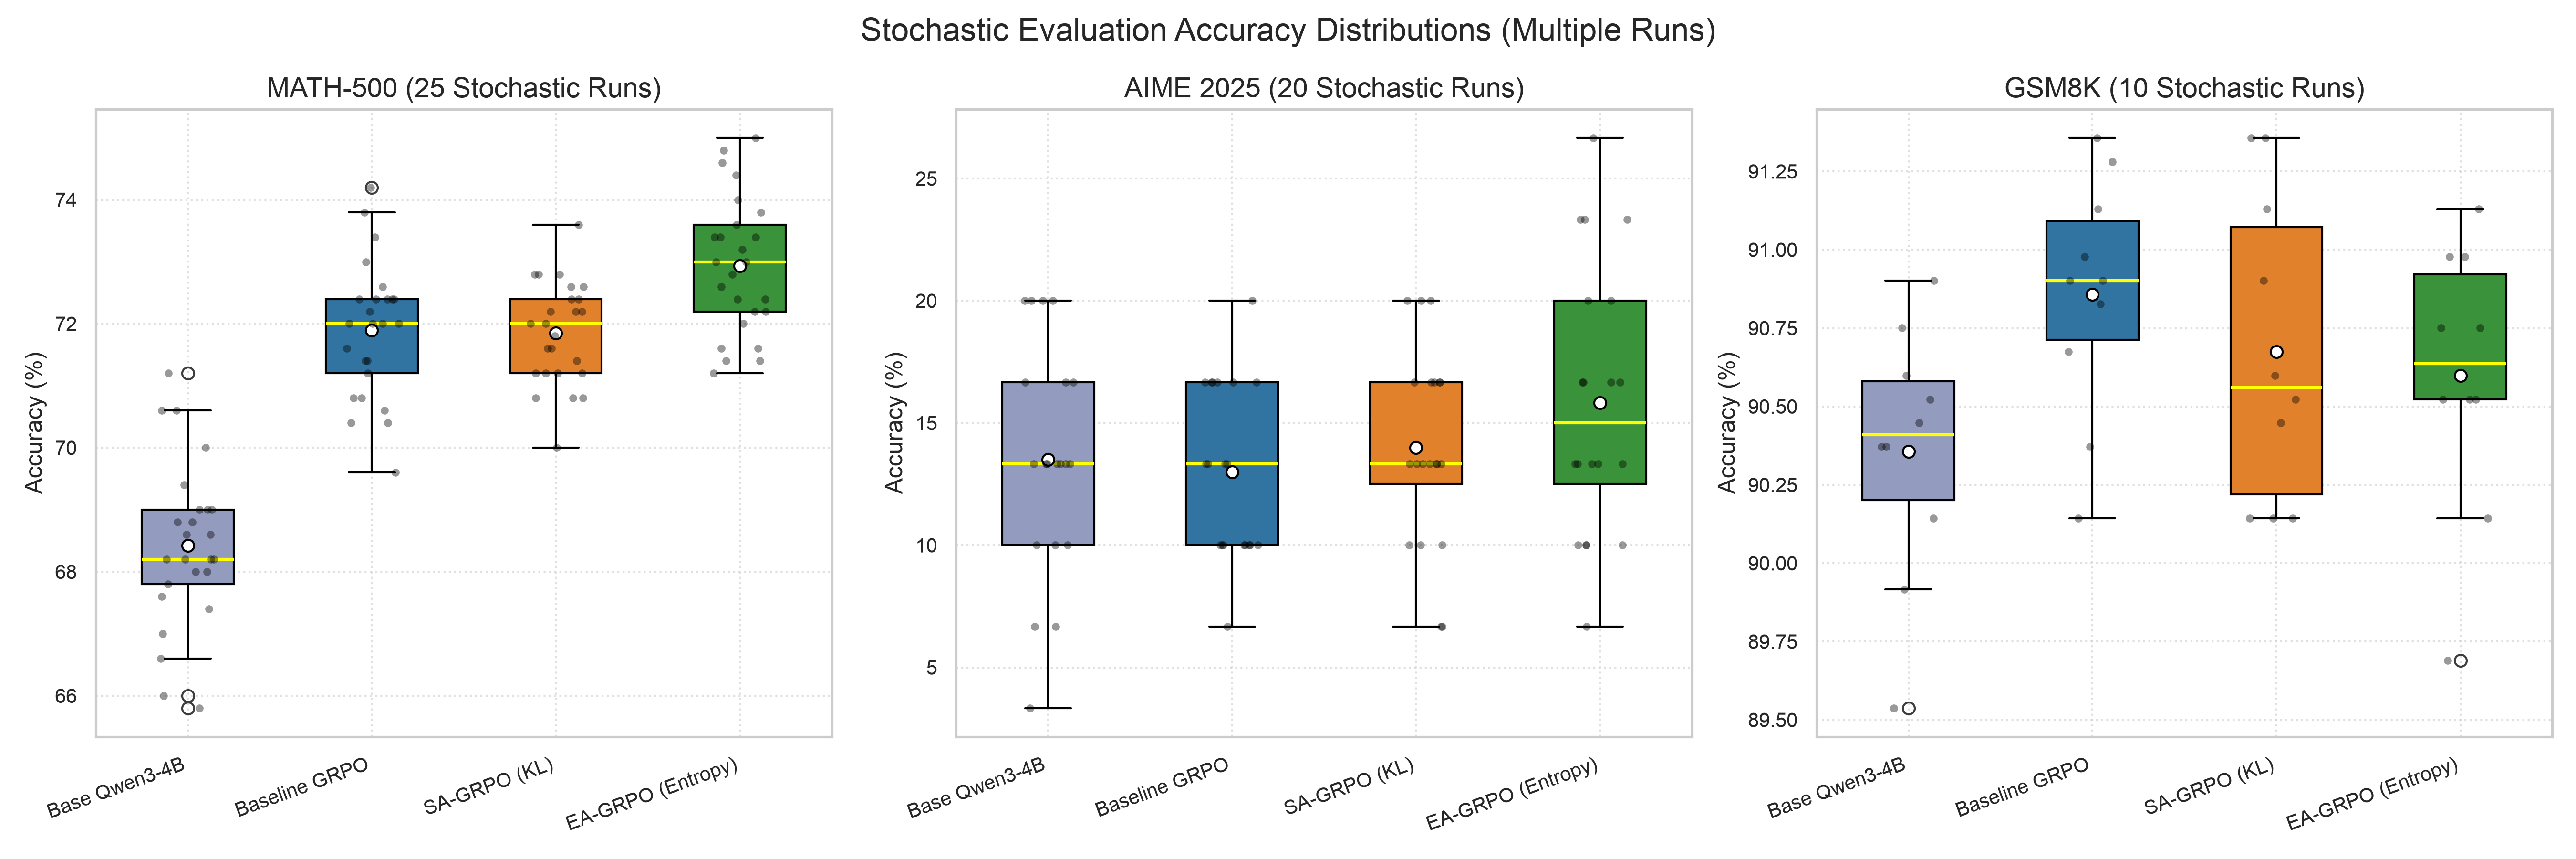
\includegraphics[width=0.9\linewidth]{images/eval_accuracy_comparison_boxplots.png}
\caption{Evaluation accuracy distributions across stochastic runs (MATH-500: 25 runs, AIME 2025: 20 runs, GSM8K: 10 runs). EA-GRPO achieves the highest median and mean on MATH-500 and AIME 2025. GSM8K is effectively saturated at $\approx$90.6\%.}
\label{fig:boxplots_app}
\end{figure}

\subsection{Problem-Wise Granular Delta Analysis}
To investigate whether accuracy gains stem from uniform incremental progress or targeted problem-solving improvements, Figure~\ref{fig:prob_diverging_app} shows the per-problem accuracy delta between EA-GRPO and Baseline GRPO across all 500 MATH-500 items, sorted ascending by difficulty level (Level 1 at top to Level 5 at bottom).

\begin{figure}[!htbp]
\centering
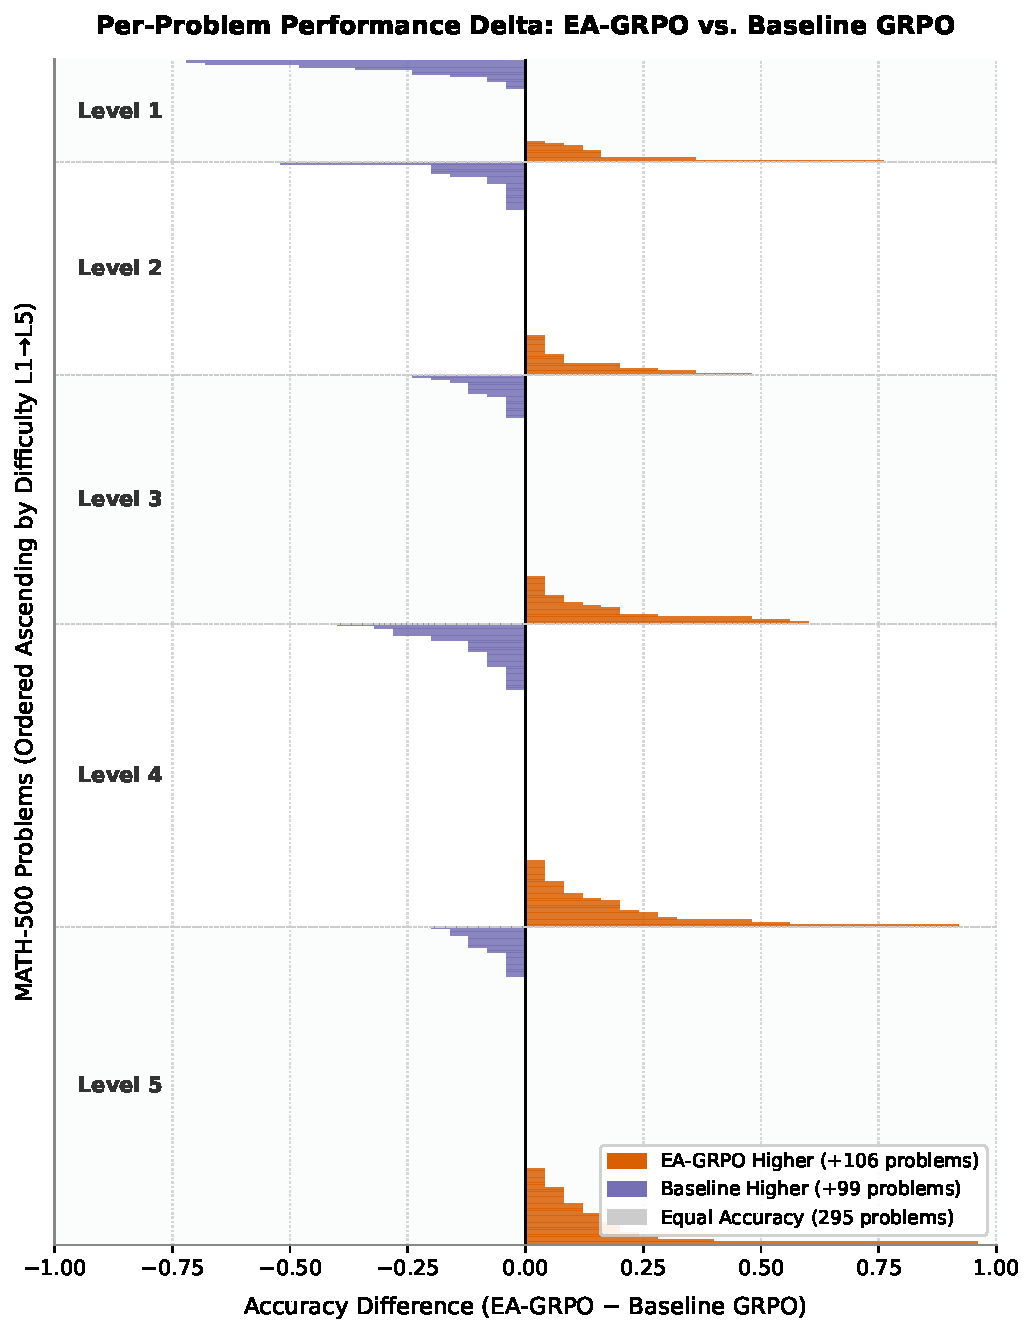
\includegraphics[width=0.88\linewidth]{images/fig_problemwise_diverging.pdf}
\caption{Per-problem accuracy difference (EA-GRPO vs. Baseline GRPO) on MATH-500 across 25 evaluation runs, ordered ascending by difficulty level (L1 to L5).}
\label{fig:prob_diverging_app}
\end{figure}

Out of 500 problems, EA-GRPO outperforms Baseline GRPO on 106 problems, Baseline GRPO leads on 99 problems, and both models achieve identical accuracy on 295 problems. Crucially, the distribution of positive deltas shifts dramatically toward higher difficulty levels: in Level 4 and Level 5, EA-GRPO dominates the rightward deltas, unlocking difficult multi-step problems that Baseline GRPO consistently fails.

\subsection{Subject-Level Accuracy Breakdown}
Table~\ref{tab:subject_app} details performance across the seven Hendrycks MATH subjects. EA-GRPO leads in four of seven subjects, with its largest margins in Number Theory (+5.03\% over Baseline) and Precalculus (+3.29\% over Baseline),domains that require precise multi-step logical chains. KL-GRPO holds the top position in Geometry (55.51\%), suggesting that KL-anchored masking better preserves spatial and coordinate reasoning chains.

\begin{table}[!htbp]
\centering
\caption{MATH-500 Accuracy by Subject (\%)}
\label{tab:subject_app}
\begin{tabular}{@{}lrcccc@{}}
\toprule
\textbf{Subject} & \textbf{N} & \textbf{Base} & \textbf{Baseline} & \textbf{KL-GRPO} & \textbf{EA-GRPO} \\
\midrule
Algebra              & 124 & 86.13 & 88.32 & 88.19 & \textbf{89.29} \\
Intermediate Algebra &  97 & 53.65 & \textbf{60.54} & 59.92 & 59.34 \\
Prealgebra           &  82 & 70.34 & \textbf{74.20} & 72.05 & 73.80 \\
Number Theory        &  62 & 80.39 & 81.68 & 85.03 & \textbf{86.71} \\
Precalculus          &  56 & 52.64 & 55.93 & 56.14 & \textbf{59.21} \\
Geometry             &  41 & 51.12 & 53.66 & \textbf{55.51} & 55.41 \\
Counting \& Prob.    &  38 & 66.63 & \textbf{69.58} & 67.79 & 69.05 \\
\bottomrule
\end{tabular}
\end{table}

\subsection{Training Dynamics and Reward Breakdown}
Figure~\ref{fig:traincurves_app} plots cumulative training accuracy over 2,001 steps. Figure~\ref{fig:reward_app} breaks down reward components over training.

\begin{figure}[!htbp]
\centering
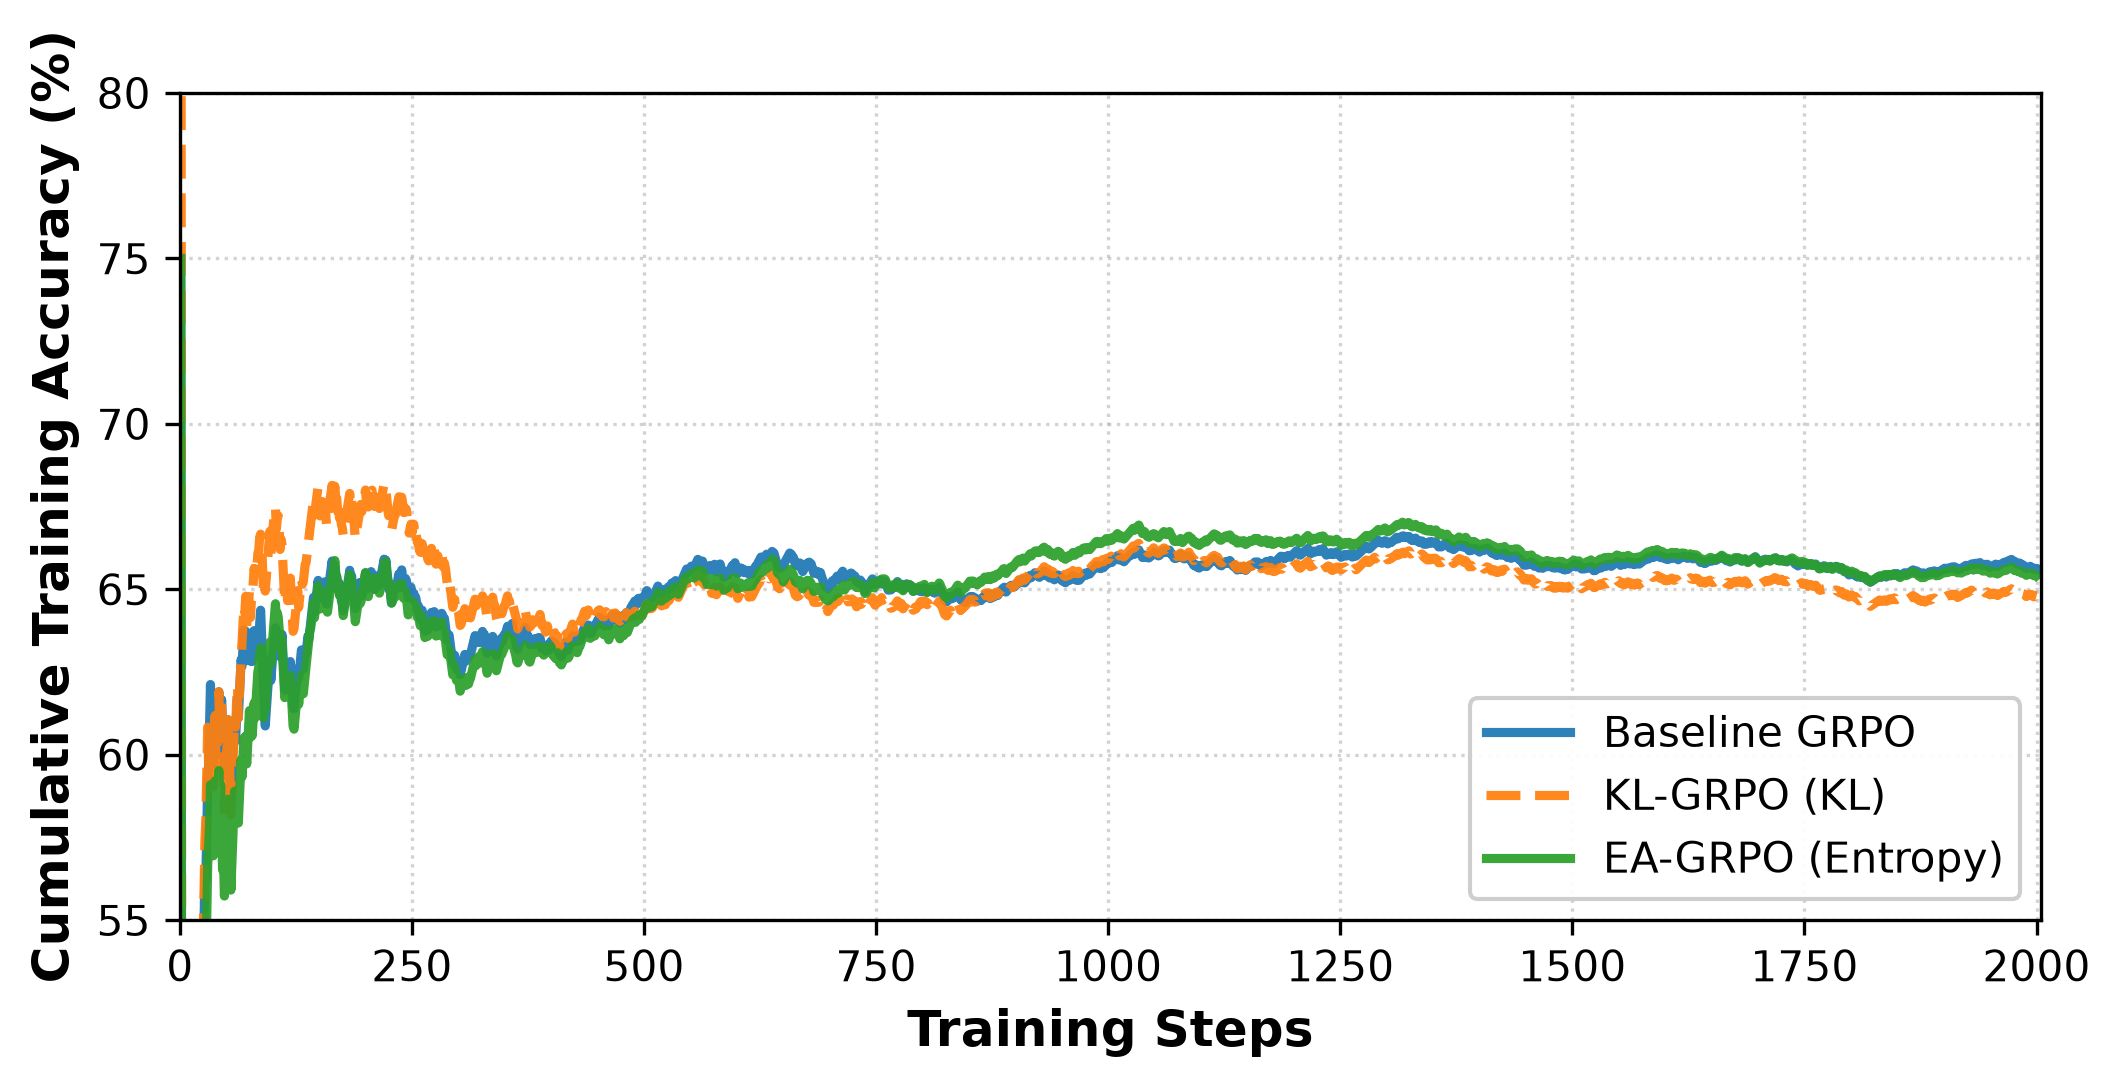
\includegraphics[width=0.85\linewidth]{images/training_accuracy_curves.png}
\caption{Cumulative training accuracy (running mean over all completions) over 2,001 steps. }
\label{fig:traincurves_app}
\end{figure}

\begin{table}[!htbp]
\centering
\caption{Training Dynamics Summary}
\label{tab:training_dynamics_app}
\begin{tabular}{@{}lccc@{}}
\toprule
\textbf{Metric} & \textbf{Baseline} & \textbf{KL-GRPO} & \textbf{EA-GRPO} \\
\midrule
Final train acc. (\%)    & \textbf{65.40} & 64.65 & 63.13 \\
Mean L2 grad norm & 0.0145 & \textbf{0.0112} & 0.0154 \\
Avg gen. length (tokens) & 517.8 & 515.7 & \textbf{527.2} \\
\bottomrule
\end{tabular}
\end{table}

\begin{figure}[!htbp]
\centering
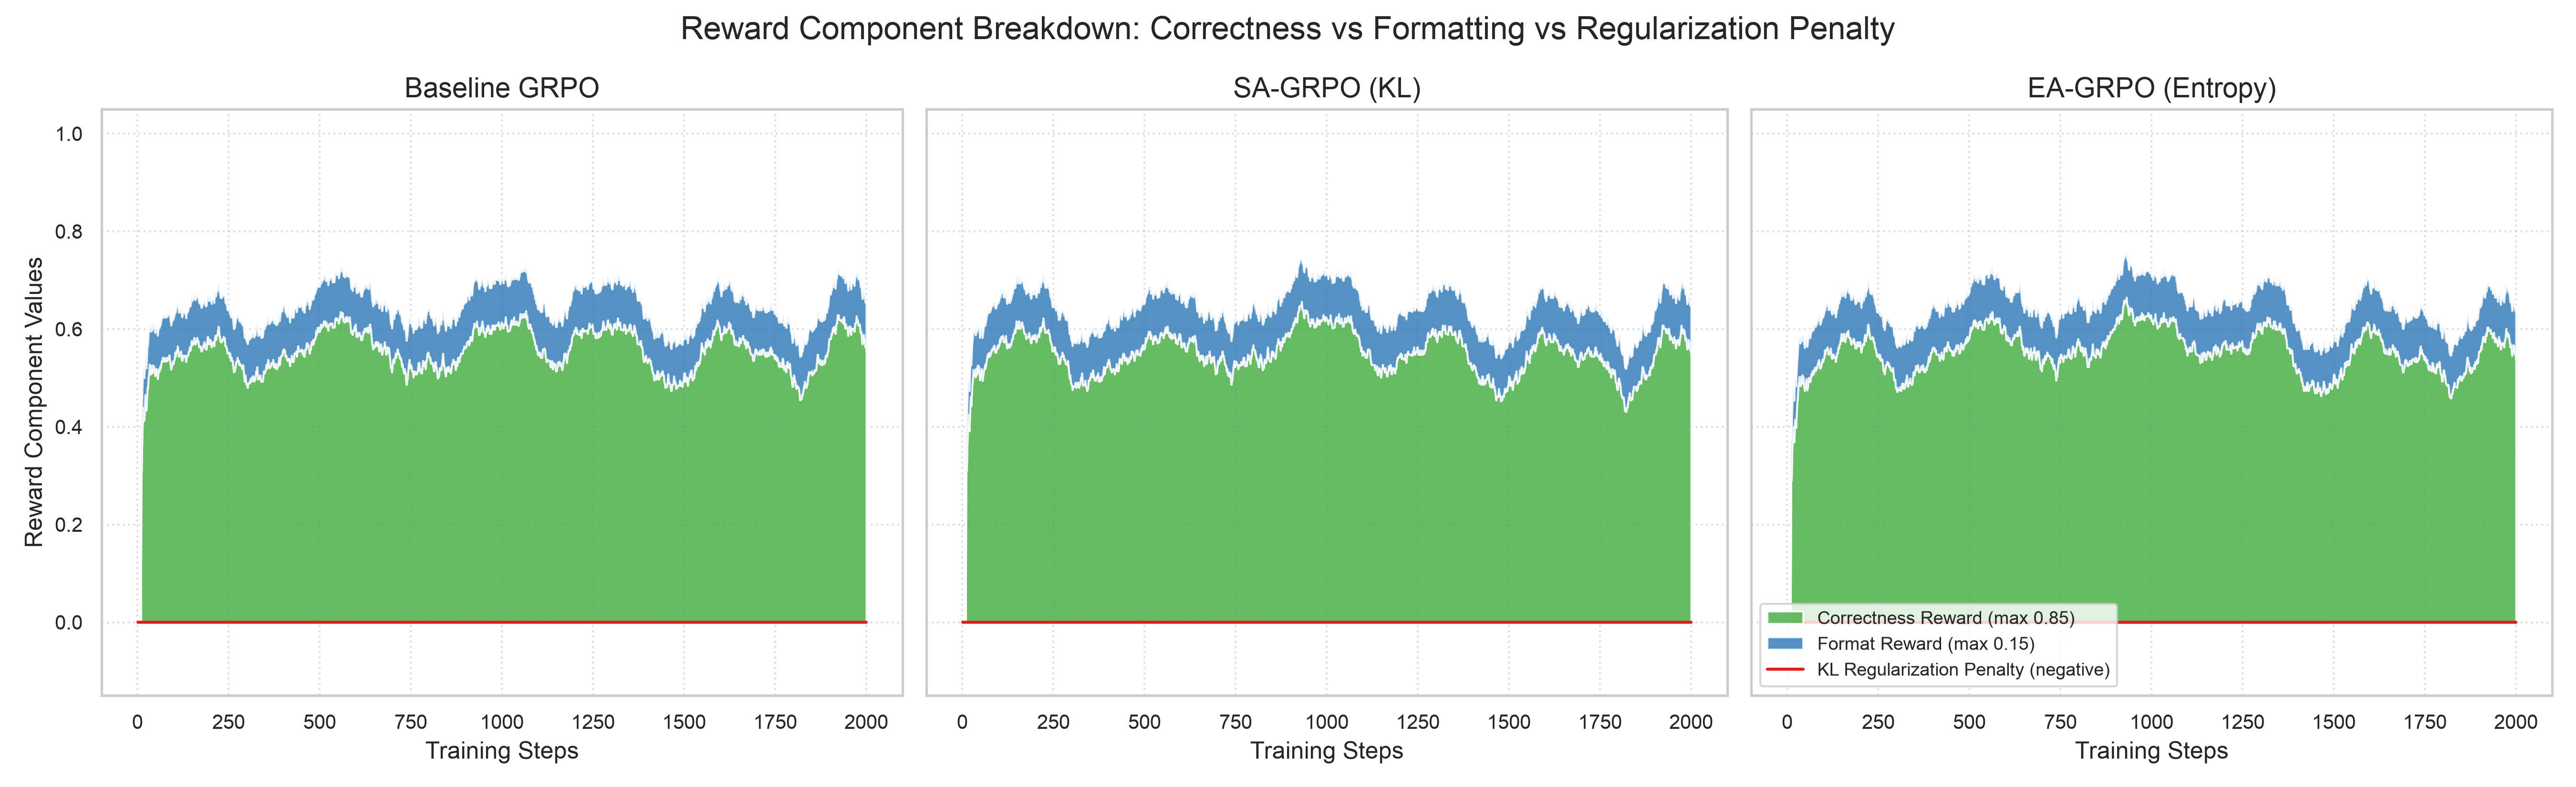
\includegraphics[width=0.88\linewidth]{images/reward_component_breakdown.png}
\caption{Reward component breakdown over training. }
\label{fig:reward_app}
\end{figure}

\subsection{Error Categorization and Newly Solved Problems}
We categorize incorrect responses into three types: truncated (hit token limit), format failures (missing \texttt{<answer>} tag), and genuinely wrong (had tag but wrong answer). KL-GRPO achieves the lowest format error rate (3.4\% of wrong responses), compared to 4.6\% for EA-GRPO and 5.5\% for Baseline GRPO.

EA-GRPO uniquely solves 6 problems (success rate $\geq$70\% of runs) that the base model fails consistently ($\leq$20\% of runs), versus 4 for KL-GRPO and 1 for Baseline GRPO. These newly unlocked problems are predominantly Level 4--5 Algebra and Number Theory problems requiring multi-step symbolic manipulation.

\subsection{Computational Cost and Masking Activation}
Figure~\ref{fig:cost_app} compares response token lengths and training step wall times. Figure~\ref{fig:masking_app} details masking gate activation rates. Table~\ref{tab:cost_format_summary} summarizes step wall times and format error rates.

\begin{table}[!htbp]
\centering
\caption{Mean Step Wall Time and Format Error Rate Summary}
\label{tab:cost_format_summary}
\begin{tabular}{lcc}
\toprule
\textbf{Variant} & \textbf{Wall Time / Step (s)} & \textbf{Format Error Rate (\%)} \\
\midrule
Baseline GRPO & 10.0 & 5.5\% \\
KL-GRPO       & 10.3 & \textbf{3.4\%} \\
EA-GRPO       & 10.1 & 4.6\% \\
\bottomrule
\end{tabular}
\end{table}

\begin{figure}[!htbp]
\centering
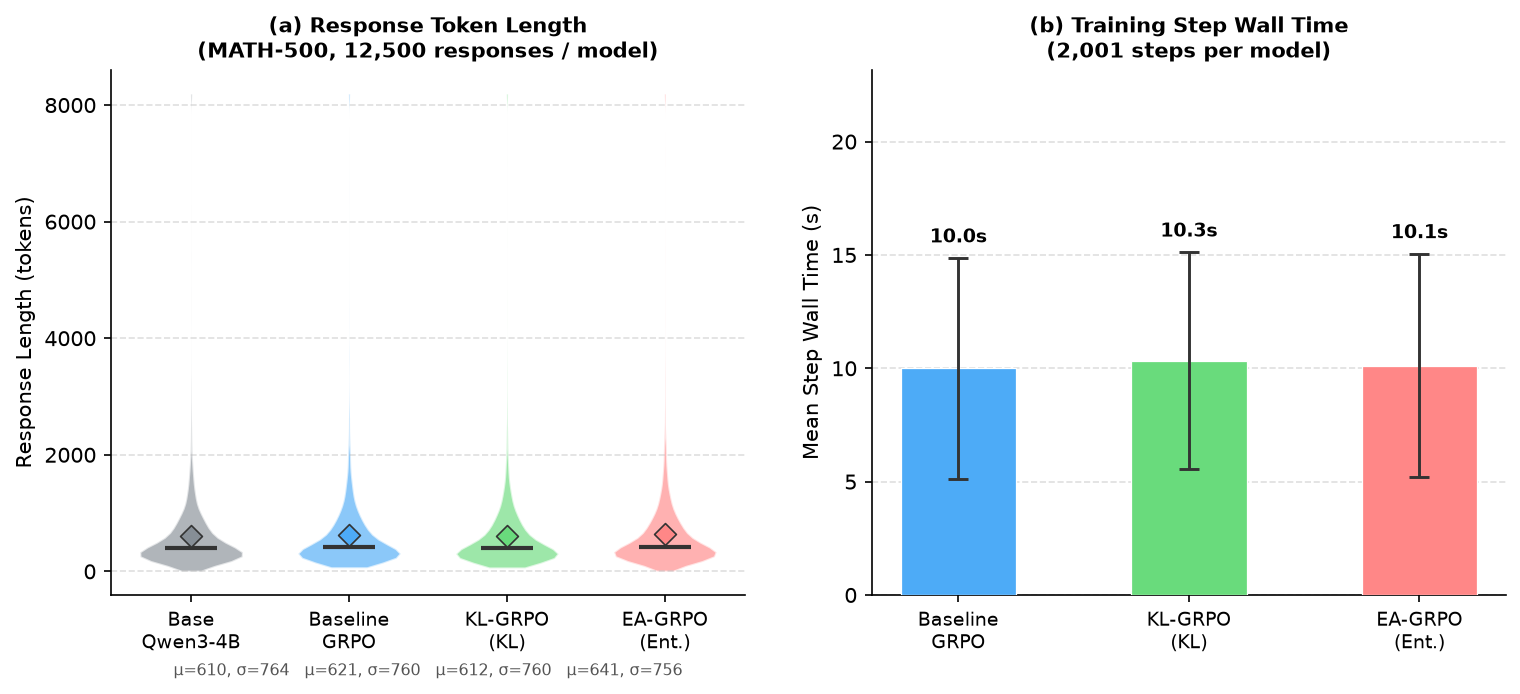
\includegraphics[width=0.82\linewidth]{images/cost_combined.png}
\caption{(a) Response token length distributions across 12,500 MATH-500 eval responses per model. (b) Mean training step wall time for fine-tuned models over 2,001 steps.}
\label{fig:cost_app}
\end{figure}

\begin{figure}[!htbp]
\centering
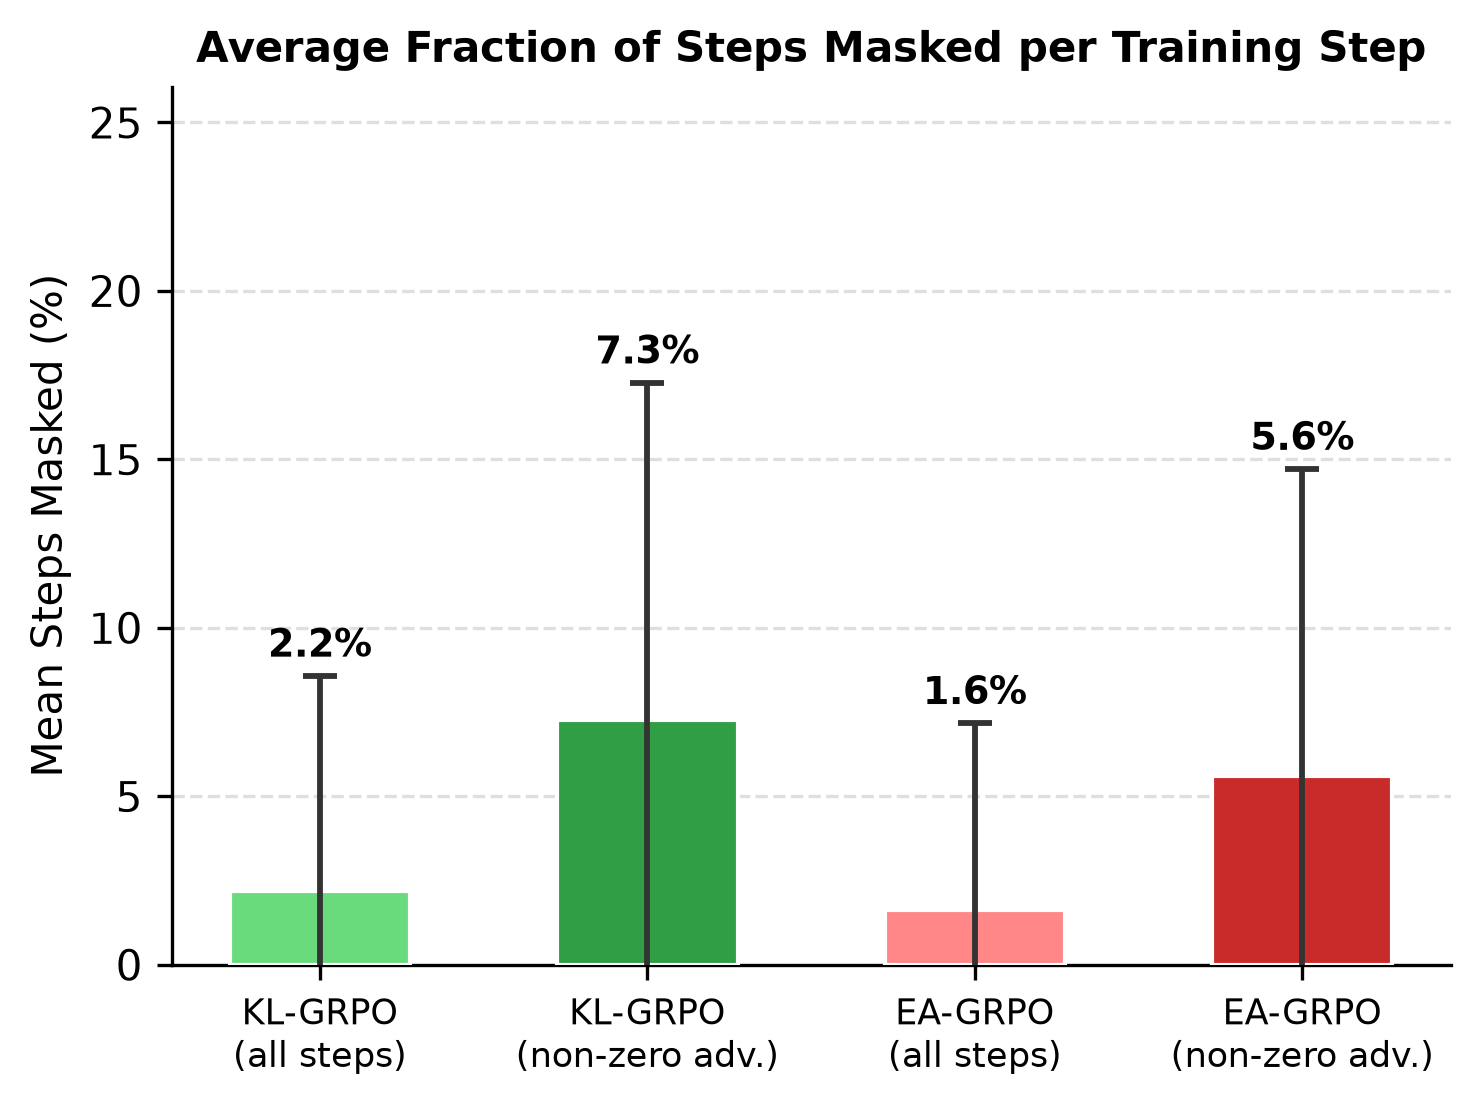
\includegraphics[width=0.72\linewidth]{images/masking_stats.png}
\caption{Average fraction of steps masked per training step for KL-GRPO and EA-GRPO, shown for all training steps and restricted to non-zero advantage steps. Error bars show $\pm$1 std dev.}
\label{fig:masking_app}
\end{figure}

\newpage
\section*{NeurIPS Paper Checklist}

\begin{enumerate}

\item {\bf Claims}
    \item[] Question: Do the main claims made in the abstract and introduction accurately reflect the paper's contributions and scope?
    \item[] Answer: \answerYes{}
    \item[] Justification: The main claims regarding step-level gradient routing, empirical accuracy gains, and training dynamics are explicitly outlined in Section 1 and supported by experiments in Section 5.
    \item[] Guidelines:
    \begin{itemize}
        \item The answer \answerNA{} means that the abstract and introduction do not include the claims made in the paper.
        \item The abstract and/or introduction should clearly state the claims made, including the contributions made in the paper and important assumptions and limitations. A \answerNo{} or \answerNA{} answer to this question will not be perceived well by the reviewers. 
        \item The claims made should match theoretical and experimental results, and reflect how much the results can be expected to generalize to other settings. 
        \item It is fine to include aspirational goals as motivation as long as it is clear that these goals are not attained by the paper. 
    \end{itemize}

\item {\bf Limitations}
    \item[] Question: Does the paper discuss the limitations of the work performed by the authors?
    \item[] Answer: \answerYes{}
    \item[] Justification: Section 6.2 explicitly details limitations regarding token vs. step granularity comparisons, threshold hyperparameter sensitivity ($\tau$), and model/dataset scalability constraints.
    \item[] Guidelines:
    \begin{itemize}
        \item The answer \answerNA{} means that the paper has no limitation while the answer \answerNo{} means that the paper has limitations, but those are not discussed in the paper. 
        \item The authors are encouraged to create a separate ``Limitations'' section in their paper.
        \item The paper should point out any strong assumptions and how robust the results are to violations of these assumptions (e.g., independence assumptions, noiseless settings, model well-specification, asymptotic approximations only holding locally). The authors should reflect on how these assumptions might be violated in practice and what the implications would be.
        \item The authors should reflect on the scope of the claims made, e.g., if the approach was only tested on a few datasets or with a few runs. In general, empirical results often depend on implicit assumptions, which should be articulated.
        \item The authors should reflect on the factors that influence the performance of the approach. For example, a facial recognition algorithm may perform poorly when image resolution is low or images are taken in low lighting. Or a speech-to-text system might not be used reliably to provide closed captions for online lectures because it fails to handle technical jargon.
        \item The authors should discuss the computational efficiency of the proposed algorithms and how they scale with dataset size.
        \item If applicable, the authors should discuss possible limitations of their approach to address problems of privacy and fairness.
        \item While the authors might fear that complete honesty about limitations might be used by reviewers as grounds for rejection, a worse outcome might be that reviewers discover limitations that aren't acknowledged in the paper. The authors should use their best judgment and recognize that individual actions in favor of transparency play an important role in developing norms that preserve the integrity of the community. Reviewers will be specifically instructed to not penalize honesty concerning limitations.
    \end{itemize}

\item {\bf Theory assumptions and proofs}
    \item[] Question: For each theoretical result, does the paper provide the full set of assumptions and a complete (and correct) proof?
    \item[] Answer: \answerNA{}
    \item[] Justification: This work is an empirical investigation of step-level gradient routing algorithms and does not present formal theoretical theorems or proofs.
    \item[] Guidelines:
    \begin{itemize}
        \item The answer \answerNA{} means that the paper does not include theoretical results. 
        \item All the theorems, formulas, and proofs in the paper should be numbered and cross-referenced.
        \item All assumptions should be clearly stated or referenced in the statement of any theorems.
        \item The proofs can either appear in the main paper or the supplemental material, but if they appear in the supplemental material, the authors are encouraged to provide a short proof sketch to provide intuition. 
        \item Inversely, any informal proof provided in the core of the paper should be complemented by formal proofs provided in appendix or supplemental material.
        \item Theorems and Lemmas that the proof relies upon should be properly referenced. 
    \end{itemize}

    \item {\bf Experimental result reproducibility}
    \item[] Question: Does the paper fully disclose all the information needed to reproduce the main experimental results of the paper to the extent that it affects the main claims and/or conclusions of the paper (regardless of whether the code and data are provided or not)?
    \item[] Answer: \answerYes{}
    \item[] Justification: Section 3 provides complete algorithmic definitions, Section 4 details exact training/eval parameters, and Appendix A outlines setup dynamics and dataset splits.
    \item[] Guidelines:
    \begin{itemize}
        \item The answer \answerNA{} means that the paper does not include experiments.
        \item If the paper includes experiments, a \answerNo{} answer to this question will not be perceived well by the reviewers: Making the paper reproducible is important, regardless of whether the code and data are provided or not.
        \item If the contribution is a dataset and\slash or model, the authors should describe the steps taken to make their results reproducible or verifiable. 
        \item Depending on the contribution, reproducibility can be accomplished in various ways. For example, if the contribution is a novel architecture, describing the architecture fully might suffice, or if the contribution is a specific model and empirical evaluation, it may be necessary to either make it possible for others to replicate the model with the same dataset, or provide access to the model. In general. releasing code and data is often one good way to accomplish this, but reproducibility can also be provided via detailed instructions for how to replicate the results, access to a hosted model (e.g., in the case of a large language model), releasing of a model checkpoint, or other means that are appropriate to the research performed.
        \item While NeurIPS does not require releasing code, the conference does require all submissions to provide some reasonable avenue for reproducibility, which may depend on the nature of the contribution. For example
        \begin{enumerate}
            \item If the contribution is primarily a new algorithm, the paper should make it clear how to reproduce that algorithm.
            \item If the contribution is primarily a new model architecture, the paper should describe the architecture clearly and fully.
            \item If the contribution is a new model (e.g., a large language model), then there should either be a way to access this model for reproducing the results or a way to reproduce the model (e.g., with an open-source dataset or instructions for how to construct the dataset).
            \item We recognize that reproducibility may be tricky in some cases, in which case authors are welcome to describe the particular way they provide for reproducibility. In the case of closed-source models, it may be that access to the model is limited in some way (e.g., to registered users), but it should be possible for other researchers to have some path to reproducing or verifying the results.
        \end{enumerate}
    \end{itemize}


\item {\bf Open access to data and code}
    \item[] Question: Does the paper provide open access to the data and code, with sufficient instructions to faithfully reproduce the main experimental results, as described in supplemental material?
    \item[] Answer: \answerYes{}
    \item[] Justification: Public Hugging Face dataset assets are cited in Section 4 and References. The full algorithm implementation details are fully specified in Section 3 and Section 4.
    \item[] Guidelines:
    \begin{itemize}
        \item The answer \answerNA{} means that paper does not include experiments requiring code.
        \item Please see the NeurIPS code and data submission guidelines (\url{https://neurips.cc/public/guides/CodeSubmissionPolicy}) for more details.
        \item While we encourage the release of code and data, we understand that this might not be possible, so \answerNo{} is an acceptable answer. Papers cannot be rejected simply for not including code, unless this is central to the contribution (e.g., for a new open-source benchmark).
        \item The instructions should contain the exact command and environment needed to run to reproduce the results. See the NeurIPS code and data submission guidelines (\url{https://neurips.cc/public/guides/CodeSubmissionPolicy}) for more details.
        \item The authors should provide instructions on data access and preparation, including how to access the raw data, preprocessed data, intermediate data, and generated data, etc.
        \item The authors should provide scripts to reproduce all experimental results for the new proposed method and baselines. If only a subset of experiments are reproducible, they should state which ones are omitted from the script and why.
        \item At submission time, to preserve anonymity, the authors should release anonymized versions (if applicable).
        \item Providing as much information as possible in supplemental material (appended to the paper) is recommended, but including URLs to data and code is permitted.
    \end{itemize}


\item {\bf Experimental setting/details}
    \item[] Question: Does the paper specify all the training and test details (e.g., data splits, hyperparameters, how they were chosen, type of optimizer) necessary to understand the results?
    \item[] Answer: \answerYes{}
    \item[] Justification: Section 4 and Table 1 provide complete lists of hyperparameters, including learning rate, batch size, group size, LoRA rank/alpha, clip thresholds, and evaluation sampling temperatures.
    \item[] Guidelines:
    \begin{itemize}
        \item The answer \answerNA{} means that the paper does not include experiments.
        \item The experimental setting should be presented in the core of the paper to a level of detail that is necessary to appreciate the results and make sense of them.
        \item The full details can be provided either with the code, in appendix, or as supplemental material.
    \end{itemize}

\item {\bf Experiment statistical significance}
    \item[] Question: Does the paper report error bars suitably and correctly defined or other appropriate information about the statistical significance of the experiments?
    \item[] Answer: \answerYes{}
    \item[] Justification: Benchmark results present standard deviation and 95\% t-distribution confidence intervals across 10--25 stochastic runs per benchmark (Section 5.1). Paired bootstrap test results ($B=10{,}000$, $p=0.0423$) are reported in Section 5.2.
    \item[] Guidelines:
    \begin{itemize}
        \item The answer \answerNA{} means that the paper does not include experiments.
        \item The authors should answer \answerYes{} if the results are accompanied by error bars, confidence intervals, or statistical significance tests, at least for the experiments that support the main claims of the paper.
        \item The factors of variability that the error bars are capturing should be clearly stated (for example, train/test split, initialization, random drawing of some parameter, or overall run with given experimental conditions).
        \item The method for calculating the error bars should be explained (closed form formula, call to a library function, bootstrap, etc.)
        \item The assumptions made should be given (e.g., Normally distributed errors).
        \item It should be clear whether the error bar is the standard deviation or the standard error of the mean.
        \item It is OK to report 1-sigma error bars, but one should state it. The authors should preferably report a 2-sigma error bar than state that they have a 96\% CI, if the hypothesis of Normality of errors is not verified.
        \item For asymmetric distributions, the authors should be careful not to show in tables or figures symmetric error bars that would yield results that are out of range (e.g., negative error rates).
        \item If error bars are reported in tables or plots, the authors should explain in the text how they were calculated and reference the corresponding figures or tables in the text.
    \end{itemize}

\item {\bf Experiments compute resources}
    \item[] Question: For each experiment, does the paper provide sufficient information on the computer resources (type of compute workers, memory, time of execution) needed to reproduce the experiments?
    \item[] Answer: \answerYes{}
    \item[] Justification: Section 4 specifies hardware resources and vLLM colocate inference settings, while Appendix A.6 and Figure 7 report exact per-step training wall-times. Experiments were conducted on a single NVIDIA L40S (48 GB) GPU hosted on RunPod.
    \item[] Guidelines:
    \begin{itemize}
        \item The answer \answerNA{} means that the paper does not include experiments.
        \item The paper should indicate the type of compute workers CPU or GPU, internal cluster, or cloud provider, including relevant memory and storage.
        \item The paper should provide the amount of compute required for each of the individual experimental runs as well as estimate the total compute. 
        \item The paper should disclose whether the full research project required more compute than the experiments reported in the paper (e.g., preliminary or failed experiments that didn't make it into the paper). 
    \end{itemize}
    
\item {\bf Code of ethics}
    \item[] Question: Does the research conducted in the paper conform, in every respect, with the NeurIPS Code of Ethics \url{https://neurips.cc/public/EthicsGuidelines}?
    \item[] Answer: \answerYes{}
    \item[] Justification: The research adheres strictly to ethical standards and double-blind anonymization guidelines.
    \item[] Guidelines:
    \begin{itemize}
        \item The answer \answerNA{} means that the authors have not reviewed the NeurIPS Code of Ethics.
        \item If the authors answer \answerNo, they should explain the special circumstances that require a deviation from the Code of Ethics.
        \item The authors should make sure to preserve anonymity (e.g., if there is a special consideration due to laws or regulations in their jurisdiction).
    \end{itemize}


\item {\bf Broader impacts}
    \item[] Question: Does the paper discuss both potential positive societal impacts and negative societal impacts of the work performed?
    \item[] Answer: \answerNA{}
    \item[] Justification: This is foundational research on reinforcement learning optimization for mathematical reasoning LLMs using public benchmarks, with no immediate direct negative societal application.
    \item[] Guidelines:
    \begin{itemize}
        \item The answer \answerNA{} means that there is no societal impact of the work performed.
        \item If the authors answer \answerNA{} or \answerNo, they should explain why their work has no societal impact or why the paper does not address societal impact.
        \item Examples of negative societal impacts include potential malicious or unintended uses (e.g., disinformation, generating fake profiles, surveillance), fairness considerations (e.g., deployment of technologies that could make decisions that unfairly impact specific groups), privacy considerations, and security considerations.
        \item The conference expects that many papers will be foundational research and not tied to particular applications, let alone deployments. However, if there is a direct path to any negative applications, the authors should point it out. For example, it is legitimate to point out that an improvement in the quality of generative models could be used to generate Deepfakes for disinformation. On the other hand, it is not needed to point out that a generic algorithm for optimizing neural networks could enable people to train models that generate Deepfakes faster.
        \item The authors should consider possible harms that could arise when the technology is being used as intended and functioning correctly, harms that could arise when the technology is being used as intended but gives incorrect results, and harms following from (intentional or unintentional) misuse of the technology.
        \item If there are negative societal impacts, the authors could also discuss possible mitigation strategies (e.g., gated release of models, providing defenses in addition to attacks, mechanisms for monitoring misuse, mechanisms to monitor how a system learns from feedback over time, improving the efficiency and accessibility of ML).
    \end{itemize}
    
\item {\bf Safeguards}
    \item[] Question: Does the paper describe safeguards that have been put in place for responsible release of data or models that have a high risk for misuse (e.g., pre-trained language models, image generators, or scraped datasets)?
    \item[] Answer: \answerNA{}
    \item[] Justification: The research utilizes standard open-weights base models and public academic datasets, posing no high-risk dual-use scenarios.
    \item[] Guidelines:
    \begin{itemize}
        \item The answer \answerNA{} means that the paper poses no such risks.
        \item Released models that have a high risk for misuse or dual-use should be released with necessary safeguards to allow for controlled use of the model, for example by requiring that users adhere to usage guidelines or restrictions to access the model or implementing safety filters. 
        \item Datasets that have been scraped from the Internet could pose safety risks. The authors should describe how they avoided releasing unsafe images.
        \item We recognize that providing effective safeguards is challenging, and many papers do not require this, but we encourage authors to take this into account and make a best faith effort.
    \end{itemize}

\item {\bf Licenses for existing assets}
    \item[] Question: Are the creators or original owners of assets (e.g., code, data, models), used in the paper, properly credited and are the license and terms of use explicitly mentioned and properly respected?
    \item[] Answer: \answerYes{}
    \item[] Justification: All assets (Qwen3-4B, MATH-500, AIME 2025, GSM8K, RLVR Math) are credited and cited in Section 4 and the References section under open research terms.
    \item[] Guidelines:
    \begin{itemize}
        \item The answer \answerNA{} means that the paper does not use existing assets.
        \item The authors should cite the original paper that produced the code package or dataset.
        \item The authors should state which version of the asset is used and, if possible, include a URL.
        \item The name of the license (e.g., CC-BY 4.0) should be included for each asset.
        \item For scraped data from a particular source (e.g., website), the copyright and terms of service of that source should be provided.
        \item If assets are released, the license, copyright information, and terms of use in the package should be provided. For popular datasets, \url{paperswithcode.com/datasets} has curated licenses for some datasets. Their licensing guide can help determine the license of a dataset.
        \item For existing datasets that are re-packaged, both the original license and the license of the derived asset (if it has changed) should be provided.
        \item If this information is not available online, the authors are encouraged to reach out to the asset's creators.
    \end{itemize}

\item {\bf New assets}
    \item[] Question: Are new assets introduced in the paper well documented and is the documentation provided alongside the assets?
    \item[] Answer: \answerNA{}
    \item[] Justification: No new dataset assets are created or released in this paper.
    \item[] Guidelines:
    \begin{itemize}
        \item The answer \answerNA{} means that the paper does not release new assets.
        \item Researchers should communicate the details of the dataset\slash code\slash model as part of their submissions via structured templates. This includes details about training, license, limitations, etc. 
        \item The paper should discuss whether and how consent was obtained from people whose asset is used.
        \item At submission time, remember to anonymize your assets (if applicable). You can either create an anonymized URL or include an anonymized zip file.
    \end{itemize}

\item {\bf Crowdsourcing and research with human subjects}
    \item[] Question: For crowdsourcing experiments and research with human subjects, does the paper include the full text of instructions given to participants and screenshots, if applicable, as well as details about compensation (if any)? 
    \item[] Answer: \answerNA{}
    \item[] Justification: No crowdsourcing or human subject experiments were performed.
    \item[] Guidelines:
    \begin{itemize}
        \item The answer \answerNA{} means that the paper does not involve crowdsourcing nor research with human subjects.
        \item Including this information in the supplemental material is fine, but if the main contribution of the paper involves human subjects, then as much detail as possible should be included in the main paper. 
        \item According to the NeurIPS Code of Ethics, workers involved in data collection, curation, or other labor should be paid at least the minimum wage in the country of the data collector. 
    \end{itemize}

\item {\bf Institutional review board (IRB) approvals or equivalent for research with human subjects}
    \item[] Question: Does the paper describe potential risks incurred by study participants, whether such risks were disclosed to the subjects, and whether Institutional Review Board (IRB) approvals (or an equivalent approval/review based on the requirements of your country or institution) were obtained?
    \item[] Answer: \answerNA{}
    \item[] Justification: No human subject research was conducted, so IRB approval is not required.
    \item[] Guidelines:
    \begin{itemize}
        \item The answer \answerNA{} means that the paper does not involve crowdsourcing nor research with human subjects.
        \item Depending on the country in which research is conducted, IRB approval (or equivalent) may be required for any human subjects research. If you obtained IRB approval, you should clearly state this in the paper. 
        \item We recognize that the procedures for this may vary significantly between institutions and locations, and we expect authors to adhere to the NeurIPS Code of Ethics and the guidelines for their institution. 
        \item For initial submissions, do not include any information that would break anonymity (if applicable), such as the institution conducting the review.
    \end{itemize}

\item {\bf Declaration of LLM usage}
    \item[] Question: Does the paper describe the usage of LLMs if it is an important, original, or non-standard component of the core methods in this research? Note that if the LLM is used only for writing, editing, or formatting purposes and does \emph{not} impact the core methodology, scientific rigor, or originality of the research, declaration is not required.
    \item[] Answer: \answerYes{}
    \item[] Justification: The proposed methods are developed and evaluated for LLM reinforcement learning. Qwen3-4B serves as the policy model, and model-generated reasoning trajectories and policy distributions are used directly in the proposed step-level masking framework.
    \item[] Guidelines:
    \begin{itemize}
        \item The answer \answerNA{} means that the core method development in this research does not involve LLMs as any important, original, or non-standard components.
        \item Please refer to our LLM policy in the NeurIPS handbook for what should or should not be described.
    \end{itemize}

\end{enumerate}

\end{document}
